%% UWAGI
%% - wszystkie pliki kodujemy w utf8
%% - stosujemy biber'a do obsługi bibliografii; nie stosujemy bibtex'a;
%%   Overleaf automatycznie wykrywa biber'a; w innych środowiskach być może
%%   będziesz musiał ustawić go ręcznie
%% - proponujemy pakiet acro do obsługi synonimów; jeśli nie widzisz potrzeby korzystania z synonimów,
%%   to zakomentuj dwie linijki w tym pliku

\documentclass[12pt, a4paper, twoside, titlepage]{report}

%%% Copyright (C) [2026] [PWr * WIT * Wydziałowa Komisja d/s Jakości Kształcenia]
%%% Zmodyfikowany i zoptymalizowany (2026)
%%% ---------------------------------------------------------------------------

%%% KONFIGURACJA EKSTRAKCJI TEKSTU (PDF COPY-PASTE)
\input{glyphtounicode} 
\pdfgentounicode=1     % Wymagane przez JSA (Jednolity System Antyplagiatowy)

%%% 1. KODOWANIE I JĘZYK
\RequirePackage[T1]{fontenc}
%\RequirePackage[utf8]{inputenc} % Opcjonalne w nowych systemach (domyślne)
\RequirePackage[english,polish]{babel} % Kolejność eng -> pl
\RequirePackage{csquotes} % Wymagane przez biblatex

%%% 2. MATEMATYKA I CZCIONKI
\RequirePackage{amsmath}
\RequirePackage{mathtools}
\RequirePackage{amsthm}
\RequirePackage{multirow}
\RequirePackage{placeins}
\RequirePackage{booktabs}
\RequirePackage{newtxtext} 
\RequirePackage{newtxmath}
\RequirePackage{microtype} % Poprawia optyczny wygląd tekstu

%%% 3. GEOMETRIA I GRAFIKA
\RequirePackage{geometry}
\geometry{
  a4paper,
  top=25mm, bottom=25mm,
  inner=25mm, outer=25mm,
  bindingoffset=5mm
}
\RequirePackage{graphicx}
\RequirePackage{xcolor}
\RequirePackage{float} % Dla opcji pozycjonowania [H]

%%% 4. NARZĘDZIA POMOCNICZE
\RequirePackage{etoolbox}

%%% 5. FORMATOWANIE TEKSTU I NAGŁÓWKÓW
\RequirePackage{titlesec}
\RequirePackage{caption}
\RequirePackage{subcaption}
\RequirePackage{setspace}

\setlength{\parindent}{0.7cm}
\setstretch{1.15} 

% Formatowanie nagłówków (Rozdział, Podrozdział)
\titleformat{\chapter}[display]
  {\bfseries\Large}
  {\chaptertitlename\ \thechapter}{0.5ex}   
  {\huge}
\titlespacing*{\chapter}{0pt}{-20pt}{20pt}

\titleformat{\section}{\bfseries\Large}{\thesection.}{1em}{}
\titlespacing*{\section}{0pt}{2.5ex plus 1ex minus .2ex}{1.3ex plus .2ex}

\titleformat{\subsection}{\bfseries\large}{\thesubsection.}{1em}{}
\titlespacing*{\subsection}{0pt}{2.25ex plus 1ex minus .2ex}{1.0ex plus .2ex}

% Numeracja ciągła wewnątrz rozdziałów
\counterwithin{figure}{chapter}
\counterwithin{table}{chapter}
\numberwithin{equation}{chapter}

% Podpisy (Captions) - pogrubione etykiety
\captionsetup{font=small, labelfont=bf, labelsep=period}

%%% 6. ALGORYTMY I LISTINGI KODU
\RequirePackage{algorithm}
\RequirePackage{algpseudocode}
\algrenewcommand\algorithmiccomment[1]{\hfill\(\triangleright\) #1}
\floatname{algorithm}{Algorytm} 

\RequirePackage{listings}
\definecolor{codebg}{RGB}{250,250,250}
\definecolor{codekw}{RGB}{0,64,160}
\definecolor{codestr}{RGB}{0,128,0}
\definecolor{codecmt}{RGB}{128,128,128}

\lstset{
  basicstyle=\ttfamily\small,
  backgroundcolor=\color{codebg},
  keywordstyle=\bfseries\color{codekw},
  stringstyle=\color{codestr},
  commentstyle=\itshape\color{codecmt},
  numbers=left,
  numberstyle=\tiny\color{gray},
  stepnumber=1,
  numbersep=8pt,
  tabsize=2,
  showstringspaces=false,
  breaklines=true,
  frame=lines,
  captionpos=b,
  % Mapowanie polskich znaków dla listings (niezbędne przy tym pakiecie)
  literate={ą}{{\k{a}}}1 {ć}{{\'c}}1 {ę}{{\k{e}}}1 {ł}{{\l{}}}1 {ń}{{\'n}}1 {ó}{{\'o}}1 {ś}{{\'s}}1 {ż}{{\.z}}1 {ź}{{\'z}}1
           {Ą}{{\k{A}}}1 {Ć}{{\'C}}1 {Ę}{{\k{E}}}1 {Ł}{{\L{}}}1 {Ń}{{\'N}}1 {Ó}{{\'O}}1 {Ś}{{\'S}}1 {Ż}{{\.Z}}1 {Ź}{{\'Z}}1
}
\renewcommand{\lstlistingname}{Listing}
\renewcommand{\lstlistlistingname}{Spis listingów}

% Styl Haskell 
\definecolor{darkgreen}{rgb}{0,0.5,0}
\lstdefinestyle{haskellStyle}{
    language=Haskell,
    commentstyle=\color{darkgreen},
    keywordstyle=\color{blue}\bfseries,
    basicstyle=\ttfamily\small,
    breaklines=true,
    stringstyle=\color{red}
}

%%% 7. HYPERREF I CLEVEREF (Musi być na końcu)
\RequirePackage[
    pdfusetitle,
    colorlinks=true,
    linkcolor=black,
    citecolor=blue,
    urlcolor=blue,
    bookmarksnumbered=true
]{hyperref}

\RequirePackage[nameinlink]{cleveref}

% Tłumaczenia dla cleveref
\crefname{figure}{Rys.}{Rys.}
\Crefname{figure}{Rysunek}{Rysunki}
\crefname{table}{Tab.}{Tab.}
\Crefname{table}{Tabela}{Tabele}
\crefname{equation}{równ.}{równ.}
\Crefname{equation}{Równanie}{Równania}
\crefname{listing}{listing}{Listingi}
\crefname{algorithm}{algorytm}{algorytmy}
\Crefname{algorithm}{Algorytm}{Algorytmy}

%%%%%%%%%%%
%% MAKRA %%
%%%%%%%%%%%

% Definicja rodzaju pracy 
\newcommand{\stRodzajPracy}{%
  \ifnum\stCzyMgr=1 MAGISTERSKA\else INŻYNIERSKA\fi
}

\newcommand{\StronaTytulowa}{
  \pagenumbering{roman}
  \sffamily
  \begin{titlepage}  
    \newgeometry{top=2.5cm, bottom=2.5cm, left=2.5cm, right=2.5cm}
    
    \begin{center}
      {\huge\bfseries Politechnika Wrocławska \par}
      \vspace{0.4cm}
      {\Large Wydział Informatyki i Telekomunikacji \par}
    \end{center}
    \par\noindent\rule{\textwidth}{1pt}\par 
    \vspace{0.5cm} 
    
    {\large
    \begin{tabular}{@{}ll}
      Kierunek: & \textbf{\stKierunek\ (\stKodKierunku)} \\
      \ifdefempty{\stSpecjalnosc}{}{Specjalność: & \textbf{\stSpecjalnosc\ (\stKodSpecjalnosci)}}
    \end{tabular}
    }
    
    \vspace*{\fill}
    
    \begin{center}
      {\huge\bfseries PRACA DYPLOMOWA \par}
      \vspace{0.3cm}    
      {\huge \stRodzajPracy \par}
      \vspace{2.0cm}
      {\Large \bfseries \stTytulPL \par} 
      \vspace{1cm}
      {\Large \stAutor \par}
      \vspace{2cm}
      {\large Opiekun pracy:\par \textbf{\stOpiekun} \par}
    \end{center}
    
    \vspace*{\fill}
    
    {\raggedright
      \small Słowa kluczowe: \textit{\stSlowaKluczowe}\par
      \vspace{0.5em}
      \par\noindent\rule{\textwidth}{1pt}\par 
    }
    
    \begin{center}
      \Large Wrocław\stRok
    \end{center}
  
    \restoregeometry
  \end{titlepage}
  \normalfont
  \cleardoublepage
  \pagestyle{empty}
}

\newenvironment{abstracts}{}{\selectlanguage{polish}\clearpage}

\newcommand{\AbstractPL}{
  \begin{center}{\Large\bfseries Streszczenie \par}\end{center}\vspace{0.5em}
}

\newcommand{\AbstractENG}{
  \selectlanguage{english}
  \begin{center}{\Large\bfseries Abstract \par}\end{center}\vspace{0.5em}
}

\newcommand{\SpisTresci}{
  \clearpage
  \addtocontents{toc}{\protect\thispagestyle{empty}} 
  \pagestyle{empty} 
  \tableofcontents
  \clearpage
  \pagestyle{empty}
}

%% WSTAWIENIE METADANYCH DO PLIKU PDF
\newcommand{\SetMetaData}{%
  \AtBeginDocument{%  
    \hypersetup{%
      pdfinfo = {%
        Title    = {\stTytulPL},
        Author   = {\stAutor},
        Subject  = {Praca dyplomowa \stRodzajPracy},  
        Keywords = {\stSlowaKluczowe}, 
        ModDate  = {\pdfcreationdate}, 
        Creator  = {pdftex}
      }
    }
  }
}
%%% KONIEC PLIKU SETTINGS.TEX % Plik z najważnieszymi ustawieniami i makrami

%% TUTAJ WPISZ DANE SWOJEJ PRACY 

\newcommand{\stKierunek}{Informatyka Techniczna}
\newcommand{\stKodKierunku}{ITE}
\newcommand{\stSpecjalnosc}{Inżynieria Systemów Informatycznych} %% zostaw pusty wpis jak nie ma specjalności
\newcommand{\stKodSpecjalnosci}{INS} %% kody kierunków i specjalności znajdziesz na stronach WIT 
\newcommand{\stCzyMgr}{0} % 1 = Magisterska, 0 = Inżynierska
\newcommand{\stTytulPL}{Inteligentna aplikacja webowa do odczytu e-booków umożliwiająca automatyczny dobór muzyki ambientowej w zależności od aktualnej treści}
\newcommand{\stTytulAng}{An intelligent web application for reading e-books that automatically selects ambient music based on the current content}
\newcommand{\stAutor}{Grzegorz Wszoła}
\newcommand{\stOpiekun}{Dr inż. Robert Wójcik}
\newcommand{\stSlowaKluczowe}{uczenie maszynowe, przetwarzanie danych, analiza emocji, analiza danych, Python}
\newcommand{\stRok}{, 2026}  % rok złożenia pracy

\SetMetaData % USTAWIENIE MATEDANYCH DLA pliku PDF

%% WŁASNE SKRÓTY
\newcommand{\IFF}{\leftrightarrow}
\newcommand{\NN}{\mathbb{N}} % liczby naturalne
\newcommand{\ZZ}{\mathbb{Z}} % liczby całkowite
\newcommand{\QQ}{\mathbb{Q}} % liczby wymierne
\newcommand{\RR}{\mathbb{R}} % liczby rzeczywiste

% Korzystamy z pakietów amsmath oraz amsthm
\newtheorem{theorem}{Twierdzenie}[chapter]
\newtheorem{lemma}{Lemat}[chapter]
\newtheorem{corollary}{Wniosek}[chapter]
\newtheorem{definition}{Definicja}[chapter]

% OBSŁUGA BIBLIOGRAFII
% STOSUJEMY biblatex ORAZ progam biber do kompilacji plików *.bib
\RequirePackage[
    backend=biber,
    style=numeric,
    sorting=none,     % Sortowanie wg kolejności występowania
    urldate=iso,      % Daty URL w formacie ISO
    seconds=true      % Pokaż sekundy w datach dostępu (opcjonalnie)
]{biblatex}
% To jest przykład zastosowania standardowego formatowania LNCS
% \usepackage[backend=biber,style=lncs]{biblatex} % styl LNCS globalnie

% Dodanie pliku z bibliografią
% TU WSTAW NAZWĘ SWOJEGO PLIKU
\addbibresource{bibliography.bib}

%% AKRONIMY (skróty;synonimy)
%%%% TUTAJ PODAJ LISTĘ SWOICH AKRONIMÓW
%%% Aby poprawnie wyświetliły wszyskie skróty
%%% należy kilka razy skompilować plik główny

\RequirePackage{acro}

%% Uważaj na formatowanie;
%% Nie zapomnij o przecinkach

\DeclareAcronym{dry}{
  short = DRY ,
  long  = Don't repeat yourself
}
\DeclareAcronym{kiss}{
  short = KISS ,
  long  = {Keep It Simple, Stupid}
}
\DeclareAcronym{sql}{
  short = SQL,
  long  = Structured Query Language
}
\DeclareAcronym{api}{
  short = API ,
  long  = Application Programming Interface,
  short-plural = APIs ,
  long-plural  = Application Programming Interfaces
}

%%%%%%%%%%%%%%%%%%%%%%%%%%%%%%%%%%%%%%%%%%%
%% NIE RUSZAJ TEGO CO JEST NIŻEJ JEŚLI  %%%
%% NIE ZNASZ ZBYT DOBRZE LATEX'A        %%%
%%%%%%%%%%%%%%%%%%%%%%%%%%%%%%%%%%%%%%%%%%%
\newcommand{\ShowAcronyms}[1]{
  \begin{center}
    {\Large\bfseries Lista skrótów \par}
  \end{center}
  \vspace{0.5em}
	
  \ifboolexpr{
      test {\ifstrequal{#1}{lof}} or
      test {\ifstrequal{#1}{toc}} or
      test {\ifstrequal{#1}{description}}
    }{%
      \printacronyms[sort=true, heading=none, template=#1]
    }{%
      \printacronyms[sort=true, heading=none, template=lof]
     }%
  \clearpage
}   % Zakomentuj tę linię, jeśli nie chcesz stosować synonimów  

%% TU ZACZYNA SIĘ DOKUMENT

\begin{document}

%% NIE RUSZAJ NASTĘPNYCH TRZECH LINIJEK %%
\StronaTytulowa
%% ZACHOWAJ STRUKTURĘ TEGO PLIKU
%% TZN. abstrakty muszą być wewnątrz środowiska abstract
%% Polecenia \AbstractPL i \AbstractENG są zdefiniowane 
%% w pliku main,tex

\begin{abstracts}
  \AbstractPL
W niniejszej pracy dyplomowej przedstawiono projekt oraz implementację aplikcaji sieciowej, która służy do czytania książek w formie elektronicznej oraz słuchania muzyki. Aplikacja dobiera dla użytkownika muzykę graną w tle na podstawie czytanego tekstu, dzięki wykorzystaniu uczenia maszynowego. System został zrealizowany przy pomocy technologi Python FastApi, React Native oraz Docker. Praca zawiera analizę wymagań realizowanego systemu, wymagania funkcjonalne zdefiniowano za pomocą diagramu i scenariuszy przypadków użycia, opisano wymagania niefunkcjonalne aplikacji oraz technologie i narzędzia wykorzystane do jej realizacji. Opisano dodatkowo sposób przedstawienia, transformacji i ujednolicenia danych. Przedstawiono metody trenowania i działanie uczenia maszynowego.
		
	\AbstractENG
This thesis presents the design and implementation of a web application for reading electronic books and listening to music. The application selects background music for the user based on the text being read, using machine learning. The system was built using Python FastAPI, React Native, and Docker technologies. The thesis includes an analysis of the system's requirements: functional requirements are defined using a use case diagram and use case scenarios, while non-functional requirements as well as the technologies and tools used in the implementation are also described. Additionally, the methods of representing, transforming, and unifying data are described. The methods of training and the operation of the machine learning model are presented.
\end{abstracts}

 % plik abstrakt.txt edytujesz samodzielnie 
\SpisTresci
\newpage
\listoffigures
\newpage
\listoftables
\newpage
\lstlistoflistings
\newpage

%%% Tutaj wyświetlamy listę akronimów
%%  jako parametr (template) możesz wybrać: lof, toc, description
%%%  
% \ShowAcronyms{lof} %% Zakomentuj tę linię jeśli nie chcesz używać synonimów

\pagenumbering{arabic}  %% NIE RUSZAJ TEGO

%% TU JEST MIEJSCE NA DOŁĄCZENIE TWOICH ROZDZIAŁÓW
\chapter{Wstęp}
\label{chapt:Wstep}

Podczas czytania książek uwaga czytelnika przykuwana jest przez sam tekst, jednak na ostateczne doświadczenie lektury wpływa wiele czynników, które na pierwszy rzut oka mogą wydawać się niepowiązane. Jednym z takich elementów jest muzyka towarzysząca czytaniu, może ona nadać ton, pogłębić odczuwany smutek lub dać poczucie lepszej immersji w świat dzieła. Celem pracy jest stworzenie systemu wspomagającego przeżywanie lektury poprzez automatyczny dobór muzyki na podstawie analizy emocjonalnej tekstu z wykorzystaniem uczenia maszynowego.

\section{Cel pracy}
Opracowanie i realizacja aplikacji webowej przeznaczonej do lektury e-booków, która w sposób
zautomatyzowany personalizuje doświadczenia użytkownika poprzez dobór podkładu muzycznego
pasującego do nastroju aktualnie odtwarzanego fragmentu tekstu. System umożliwi analizę treści w
czasie rzeczywistym, wykorzystując modele uczenia maszynowego do klasyfikacji emocjonalnej tekstu
i dynamicznego sterowania odtwarzaczem audio. Zastosowanie do implementacji rozwiązania
nowoczesnych technologii (React.js, FastAPI/Python), architektury REST API oraz kontenerów
Docker, co zapewni skalowalność systemu i ułatwi jego wdrożenie.

\section{Aspekt inżynierski}
Projekt oraz implementacja uniwersalnej aplikacji do odczytu e-booków umożliwiającej automatyczny
dobór muzyki ambientowej w zależności od aktualnie prezentowanej treści. Realizacja pełnego stosu
technologicznego (full-stack) systemu: warstwy prezentacji (technologia React.js lub alternatywna) -
zapewnia interfejs czytnika obsługujący formaty EPUB/PDF; logiki biznesowej (technologia
FastAPI/Python) - integruje potok przetwarzania języka naturalnego (NLP), w którym model Sentence
Transformer dokonuje ekstrakcji cech tekstu (embedding), a wytrenowany klasyfikator
XGBoost/LightGBM przypisuje mu określony nastrój; warstwy danych - optymalizacja wydajności
aplikacji poprzez udostępnianie informacji o utworach w relacyjnej bazie SQLite, natomiast plików
audio za pośrednictwem wydajnego serwera statycznego Nginx. Podejmowanie decyzji o zmianie
ścieżki dźwiękowej na podstawie analizy statystycznej wyjścia modelu (thresholding) oraz dokonanej
oceny poziomu emocjonalnego aktualnie odtwarzanego fragmentu tekstu (eliminacja zbyt częstych
zmian muzyki). Wdrożenie systemu z użyciem technologii Docker oraz środowiska Docker Compose
(izolacja usług i ułatwienie zarządzania zależnościami). Weryfikacja poprawności działania aplikacji z
wykorzystaniem testów jednostkowych, integracyjnych i funkcjonalnych E2E. Analiza wyników testów
oraz wnioski. 

\section{Wykorzystanie AI}
W trakcie realizacji pracy wykorzystano modele językowe Claude Sonnet (Anthropic) oraz Gemini (Google) jako wsparcie w procesie tworzenia oprogramowania i redagowania dokumentacji. Narzędzia te były używane w szczególności do: wyszukiwania i syntezy informacji na temat wykorzystywanych technologii (React, FastAPI, biblioteki uczenia maszynowego); wsparcia w roli asystenta programisty (\textit{pair programming}) przy pisaniu fragmentów kodu, które następnie były dogłębnie analizowane, testowane i w razie potrzeby modyfikowane. Nauki nowych technologii i wcześniej nieznanych wzorców projektowych. Generowania wstępnych szkiców dokumentacji technicznej kodu oraz propozycji scenariuszy testowych, które zostały zweryfikowane i dostosowane do rzeczywistych wymagań systemu. Cały kod źródłowy został napisany samodzielnie lub zredagowany po dogłębnym zrozumieniu jego działania.

\chapter{Analiza istniejących aplikacji do odczytu e-booków}

Analizie poddane zostały darmowe aplikacje desktopowe (Calibre) oraz przeglądarkowe (Readest, Flow) pod względem:
\begin{itemize}
    \item Obsługiwanych formatów.
    \item Interfejsu graficznego (UI) oraz łatwości użytkowania (UX).
    \item Technologii wyróżniających poszczególne aplikacje
\end{itemize}

Kryterium wyboru aplikacji do analizy stanowiła ich popularność wśród 
użytkowników, liczba pozytywnych recenzji oraz łatwy dostęp (brak wymaganego logowania lub zakładania konta). Wybrane aplikacje reprezentują dwa odmienne modele dystrybucji oprogramowania, klasyczne programy instalowane lokalnie oraz rozwiązania działające bezpośrednio w przeglądarce internetowej, co pozwala na porównanie różnych podejść do problemu odczytu e-booków.

\section{Calibre}
Calibre jest jedną z najbardziej rozbudowanych aplikacji do odczytu treści w formie elektronicznej. Według instrukcji użytkowania \cite{CalibreUserManual}, aplikacja umożliwia między innymi wyświetlanie, przetwarzanie i katalogowanie treści. Z bardziej zaawansowanych funkcjonalności daje możliwość pobierania metadanych z internetu, lub z dostępnych gazet tworzenia książek elektronicznych.

Jej ograniczeniami jest dość przestarzały i na pierwszy rzut oka skomplikowany interfejs. Duża część obsługiwanych formatów oraz funkcji jest bardzo specjalistyczna i nie dotyka problemów większości użytkowników.

Calibre pozostaje jednak najbardziej wszechstronnym narzędziem spośród analizowanych aplikacji desktopowych, szczególnie w kontekście zarządzania większą biblioteką elektroniczną.

\section{Flow}
Flow to aplikacja przeglądarkowa pozwalająca na czytanie książek elektronicznych w formacie EPUB. Wyróżnia się ona szczególnie interfejsem zbliżonym do Visual Studio Code, a wypisane przez twórców funkcjonalności \cite{Flow} to między innymi, zaawansowane i szybkie wyszukiwanie w książce, podgląd obrazów, pamięć w chmurze, czy spersonalizowane motywy.
\newpage
Jest o wiele mniej rozbudowana niż dla przykładu Calibre, jednak łatwość i jakość samego użytkowania są na wysokim poziomie. Interfejs szczególnie może podobać się osobom na codzień korzystającym z Visual Studio Code, a personalizowane motywy dają szeroki wybór dla każdego użytkownika. Dużą korzyścią jest również pamięć w chmurze dzięki której nie wymagane jest wgrywanie tej samej książki od nowa za każdym razem.

Podobnie jak w przypadku pozostałych analizowanych aplikacji, Flow nie oferuje żadnych funkcjonalności opartych na sztucznej inteligencji ani uczeniu maszynowym personalizacja ogranicza się do warstwy wizualnej (motywy, typografia) oraz podstawowych narzędzi organizacyjnych (biblioteka, zakreślanie, wyszukiwanie).

\section{Readest}
Readest \cite{Readest} jest aplikacją przeglądarkową, ale posiada również wersje mobilne na telefony z systemem IOS (Apple) i Adnroid jak i również wersje na komputery z systemem operacyjnym MacOs, Linux i Windows. Wersja przeglądarkowa posiada nowoczesny i przyjemny w użytkowaniu interfejs opierający się głównie na ikonach.

Posiada zbliżone funkcjonalności do Flow, jak odczytywanie książek elektronicznych w formacie EPUB oraz PDF, przeglądanie rozdziałów, wyszukiwanie w tekście. Z bardziej rozbudowanych funkcji umożliwia również dynamicznie tłumaczenie tekstu i możliwość czytania dwóch tekstów jednocześnie.

Spośród wszystkich analizowanych aplikacji, Readest jako jedyna wykorzystuje mechanizmy sztucznej inteligencji nie tylko do syntezy mowy, ale i planuje rozwój w kierunku podsumowań tekstu generowanych przez AI (funkcja w fazie rozwoju). Stanowi to istotny punkt odniesienia w kontekście niniejszej pracy, ponieważ pokazuje rosnące zainteresowanie integracją komponentów ML/AI w tradycyjnie prostych narzędziach do czytania e-booków, jednak wciąż w sposób ograniczony do pojedynczych funkcji pomocniczych, a nie stanowiący centralny element aplikacji.

\section{Podsumowanie}
Po analizie dostępnych na rynku aplikacji Calibre, Readest oraz Flow, łatwo można zauważyć wspólny mianownik, którym jest skupienie na funkcjach związanych z zarządzaniem treścią oraz personalizacją wyglądu. Przeprowadzona ewaluacja pokazuje, że na rynku brakuje aplikacji łączących odczyt e-booków z zaawansowanymi funkcjami opartymi na sztucznej inteligencji i uczeniu maszynowym.

W kontekście niniejszej pracy warto wspomnieć o aplikacji MoodReads \cite{MoodeReads}, która najbardziej zbliża się do problematyki poruszanej w poniższym projekcie, dobierając muzykę do czytanej książki. Rozwiązanie to nie analizuje jednak treści na bieżąco, dobór utworów opiera się wyłącznie na gatunku literackim całej książki, a nie na emocjonalnym charakterze aktualnie czytanego fragmentu, co znacząco ogranicza precyzję i dynamikę dopasowania.
\newpage
Przeprowadzona analiza wykazała istotną lukę na rynku aplikacji do odczytu treści elektronicznych w zakresie integracji uczenia maszynowego z analizą emocjonalną tekstu w czasie rzeczywistym. Stanowi to uzasadnienie dla zaprojektowania i implementacji rozwiązania opisanego w niniejszej pracy, w którym dobór muzyki ambientowej nie opiera się na statycznych metadanych, lecz na dynamicznej analizie emocjonalnej treści czytanego tekstu.

\chapter{Analiza emocji i transformacja zbiorów danych}

Dobór odpowiedniego zbioru danych \textit{(ang. dataset)} jest jedną z kluczowych decyzji
podczas pracy z modelami uczenia maszynowego. Dobrze dobrane dane mogą znacząco poprawić jakość
modelu. Z kolei ich nieumiejętne przetwarzanie lub niedopasowanie domeny danych do zadania (np.
trenowanie modelu generującego poezję na tekstach prozatorskich) prowadzi do błędów i
pogorszenia wyników, które często trudno wykryć.

\begin{figure}[h]
    \centering
    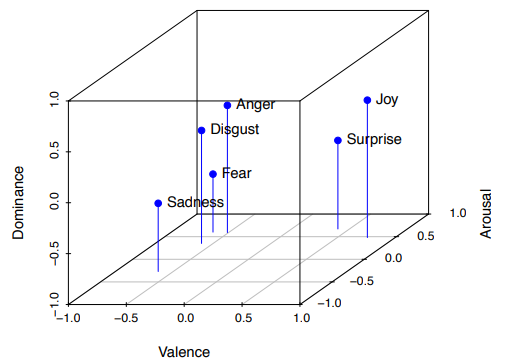
\includegraphics[width=0.7\linewidth]{figures/3/vad.png}
    \caption[Przestrzeń afektywna rozpięta przez trzy wymiary VAD wraz z położeniem sześciu
    podstawowych emocji Ekmana]{Przestrzeń afektywna rozpięta przez trzy wymiary VAD wraz z
    położeniem sześciu podstawowych emocji Ekmana, wyznaczonym przez Russella i Mehrabiana. Źródło:
    \cite{buechel-hahn-2017-emobank}, na podstawie:~\cite{russel_james_evidence}}
    \label{fig:vad_representation}
\end{figure}

\section{Czym jest VAD}
VAD (ang. Valence, Arousal, Dominance) jest wymiarowym modelem emocji, w którym stan emocjonalny
reprezentowany jest przez trzy wartości liczbowe. Wartościowość (ang. \textit{valence}) określa,
jak przyjemna lub nieprzyjemna jest dana emocja, pobudzenie (ang. \textit{arousal}) jak silnie
aktywuje ona organizm, a dominacja (ang. \textit{dominance}) w jakim stopniu osoba odczuwa
kontrolę nad sytuacją. Dzięki temu można odróżnić emocje podobne pod względem walencji i
pobudzenia, np. gniew (wysoka dominacja) od strachu (niska dominacja). W skrócie pozwala opisać
emocje jako punkt w trójwymiarowym ciągłym systemie, gdzie osiami są właśnie te parametry
\cite{vad_description}.

Podejście wymiarowe ma kilka przewag nad modelami dyskretnymi, w których emocji przypisuje się
jedną z ustalonych etykiet. Ze względu na ciągłość skali VAD pozwala opisać nie tylko konkretną
emocję, lecz także jej intensywność oraz stany pośrednie. Dodatkowo wartości liczbowe
umożliwiają wykonywanie podstawowych operacji statystycznych, np. uśrednienie dwóch ocen, co w
przypadku etykiet jest utrudnione lub wymaga dodatkowych założeń. Wadą tego podejścia jest jednak
mniejsza intuicyjność, ponieważ trójka liczb jest trudniejsza do zinterpretowania niż nazwa
emocji.

\section{NRC VAD leksykon}
\label{sec:nrc_vad}
NRC VAD Lexicon v2 jest jednym z największych zasobów opisujących emocje w ujęciu wymiarowym.
Zawiera ponad 55 tysięcy angielskich słów oraz wyrażeń wielowyrazowych, z których każdemu
przypisano trzy wartości (walencję, pobudzenie i dominację) na skali od $-1$ do $1$. Oceny
pochodzą od ankietowanych i zostały zebrane metodą \textit{Best-Worst Scaling}, w której
respondent spośród kilku terminów wybiera ten o największej i najmniejszej wartości danego
wymiaru. Daje to bardziej spójne wyniki niż bezpośrednie ocenianie na skali liczbowej.
Szczegółowy opis procesu zbierania danych i jego rzetelności można znaleźć w
pracy~\cite{mohammad2025nrcvadlexiconv2}.

Leksykon NRC VAD nie sprawdza się jako bezpośredni zbiór treningowy. Zawiera on pojedyncze słowa
i krótkie frazy, więc model trenowany na takich danych nie nauczyłby się uwzględniać kontekstu
zdania. Alternatywą jest użycie leksykonu do zbudowania reprezentacji wejściowej zamiast modelu
osadzeń zdań (ang. \textit{sentence embedding model}), na przykład przez uśrednienie wartości
VAD słów występujących w tekście. Takie podejście, nazywane workiem słów (ang. \textit{bag of
words}), ma jednak tę wadę, że pomija kolejność słów, wieloznaczność i negację. Wyniki
eksperymentów (Tabela~\ref{tab:wyniki_vad}) pokazują, że zamrożony model osadzeń zdań (ang.
\textit{frozen sentence embedder}) osiąga znacznie niższy błąd niż podejście oparte na
leksykonie. % TODO: wstawić liczby i metrykę

\section{EmoBank}
EmoBank~\cite{buechel-hahn-2017-emobank} to zbiór około 10 tysięcy angielskich zdań, z których
każde oceniono w wymiarach VAD na skali od 1 do 5. Oceny wystawiali ankietowani, a autorzy
zbioru zbadali m.in. wpływ perspektywy adnotacji (emocje wyrażane przez autora tekstu a emocje
odczuwane przez czytelnika) na uzyskane wyniki. Szczegóły dotyczące procesu zbierania i
weryfikacji danych opisano w pracy źródłowej.

W porównaniu z leksykonem NRC VAD, EmoBank jest lepiej dopasowany do zadania, ponieważ etykiety
przypisano całym zdaniom, a nie pojedynczym słowom. Ograniczeniem jest jednak skład domenowy
zbioru (Tabela~\ref{tab:emobank_genres}). Fikcja stanowi jedynie około jednej czwartej danych,
a pozostałe zdania pochodzą z tekstów takich jak wiadomości, listy czy przewodniki turystyczne,
co może negatywnie wpłynąć na wynik modelu. Dodatkowo zdania oceniano pojedynczo, bez kontekstu
sąsiednich fragmentów, a w czytaniu książki nastrój zależy właśnie od szerszego fragmentu.

\begin{table}[htbp]
  \centering
  \caption[Rozkład gatunków w zbiorze EmoBank]{Rozkład gatunków tekstu w zbiorze
  EmoBank przed i po filtrowaniu. SE07 oznacza korpus nagłówków prasowych
  z zadania SemEval-2007 (\textit{Affective Text}), a MASC --- zróżnicowany
  gatunkowo podzbiór korpusu OANC (\textit{Manually Annotated Sub-Corpus}).
  Źródło: \cite{buechel-hahn-2017-emobank}.}
  \label{tab:emobank_genres}
  \begin{tabular}{llrr}
    \toprule
    Korpus & Domena & Surowe & Po filtrowaniu \\
    \midrule
    SE07 & nagłówki wiadomości & 1250 & 1192 \\
    \midrule
    \multirow{6}{*}{MASC} & blogi & 1378 & 1336 \\
     & eseje & 1196 & 1135 \\
     & fikcja & 2893 & 2753 \\
     & listy & 1479 & 1413 \\
     & gazety & 1381 & 1314 \\
     & przewodniki turystyczne & 971 & 919 \\
    \midrule
    \multicolumn{2}{l}{\textbf{Suma}} & \textbf{$10\,548$} & \textbf{$10\,062$} \\
    \bottomrule
  \end{tabular}
\end{table}

\FloatBarrier
\section{CR4-NarrEmote}
CR4-NarrEmote to zbiór, który zawiera ponad $200\,000$ adnotacji wykonanych przez ponad $3\,500$ 
osób, przy czym każda adnotacja dotyczy pojedynczego zdania~\cite{piper-budac-2025-cr4}. Największą
zaletą jest pochodzenie tekstów. Popularne
zbiory, takie jak GoEmotions~\cite{GoEmotions} (komentarze z serwisu Reddit) czy
EmoBank~\cite{buechel-hahn-2017-emobank}, opierają się w większości na krótkich formach, a nie
na literaturze narracyjnej. Autorzy CR4-NarrEmote opisują źródło zdań następująco: \textit{„Skupiamy
się na dłuższych formach narracyjnych z dwunastu różnych gatunków literatury pięknej i faktu,
fragmentach obejmujących okres ostatnich 150 lat oraz tekstach pochodzących z różnych obszarów
kulturowych kręgu anglojęzycznego, w tym z Nigerii, Indii i Afryki Południowej, a także z Ameryki
Północnej”} (tłum. własne)~\cite[s.~9774]{piper-budac-2025-cr4}. Ponieważ aplikacja analizuje
fragmenty książek elektronicznych, dopasowanie domeny danych treningowych do
domeny użycia jest tu kluczowe.

Uczestnicy oceniali zdania, wybierając dowolną etykietę emocji (nie byli
ograniczeni zamkniętym zbiorem). Podane etykiety zostały następnie
przekształcone na wartości VAD w skali od $0$ do $1$ z użyciem leksykonu NRC
VAD (sekcja~\ref{sec:nrc_vad}), a potem przeskalowane do przedziału od $-1$
do $1$:
\[
X_{\text{scaled}} = \operatorname{round}(2X - 1,\ 4),
\]
gdzie $X$ oznacza wartość z przedziału $[0, 1]$.
Autorzy udostępniają trzy wersje mapowania etykiet na VAD. Pierwsza (NRC) opiera
się wyłącznie na leksykonie NRC, co zapewnia spójność, ale pomija kontekst:
\textit{„Podejście to, pomimo swojej spójności, posiada braki w reprezentacji
kontekstu (np. wszystkie formy słowa «miłość» są traktowane tak samo)”}
(tłum. własne)~\cite[s.~9775]{piper-budac-2025-cr4}. Druga (NRCBERT) łączy etykietę
nadaną przez uczestnika z kontekstem zdania, wykorzystując Sentence-BERT
(SBERT)~\cite{reimers-gurevych-2019-sbert}. Trzecia (EMO) polega na wytrenowaniu
modelu regresyjnego na reprezentacjach SBERT, bez użycia etykiet uczestników.

Rozkłady wartości uzyskanych poszczególnymi metodami przedstawia
rysunek~\ref{fig:distribution_VAD}. Mapowanie oparte wyłącznie na leksykonie
NRC daje najszerszy rozkład we wszystkich trzech wymiarach, natomiast
wersja trzecia (oznaczona na wykresie jako EMO) jest silnie skupiona wokół
wartości neutralnej, szczególnie dla pobudzenia i dominacji. Wersja druga
(NRCBERT) zajmuje pozycję pośrednią.

\begin{figure}[htbp]
  \centering
  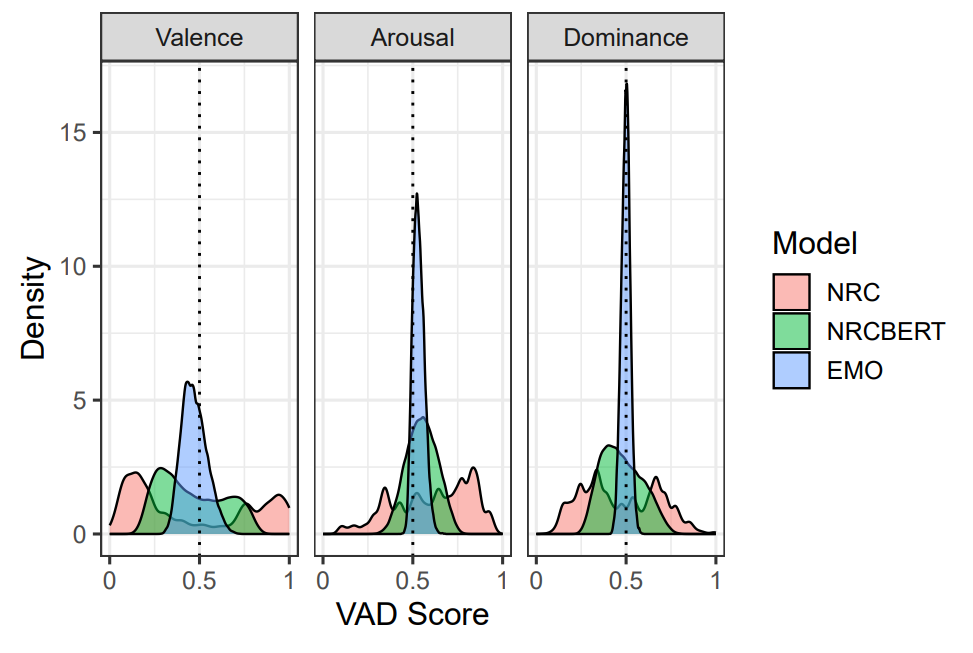
\includegraphics[width=0.8\linewidth]{figures/3/vad_score.png}
  \caption{Rozkłady wartościowości, pobudzenia i dominacji (VAD) dla trzech
  metod mapowania etykiet na wartości VAD. Linia przerywana oznacza wartość
  neutralną~(0,5). Opracowanie na podstawie~\cite[s.~9776]{piper-budac-2025-cr4}.}
  \label{fig:distribution_VAD}
\end{figure}

\FloatBarrier
\subsection{Własna transformacja danych i rekomendacje autorów}
Do trenowania modelu autorzy zalecają użycie wersji drugiej (SBERT oraz etykiety użytkowników) w
przypadku wartościowości (ang. \textit{valence}), oraz pierwszej (mapowania za pomocą leksykonu) 
wersji dla pobudzenia (ang. \textit{arousal}) oraz dominacji (ang. \textit{dominance}):
\textit{„Rekomendujemy użycie NRC dla zadań z pobudzeniem oraz dominacją, jednak dla 
bardziej zbalansowanego przewidywania wartościowości polecamy predykcje NRCBERT”} (tłum.~własne)
~\cite[s.~9776]{piper-budac-2025-cr4}. Podczas badań każdy z badanych mógł opisać dane zdanie
więcej niż jedną emocją, dlatego dla trenowania swojego modelu kilka adnotacji w ramach jednego
zdania przez jednego badanego musiały zostać uśrednione. Według zaleceń autorów do trenowania
modelu zostały użyte BERT\_V, oraz A i D pochodzące z NRC. Finalny zbiór danych użyty do trenowania,
testowania i porównania modeli wyglądał następująco:

\begin{table}[htbp]
  \centering
  \caption{Przykładowe rekordy ze zbioru danych zawierające pierwotne wartości VAD oraz wyznaczone BERT\_V}
  \label{tab:vad_bert_v_sample}
  \begin{tabular}{lrrrrl}
    \toprule
    \textbf{ID tekstu} & \textbf{V} & \textbf{A} & \textbf{D} & \textbf{BERT\_V} & \textbf{Treść tekstu} \\
    \midrule
    100116072 & $-0,6320$ & $0,4980$ & $-0,3627$ & $-0,3724$ & I shouted for her... \\
    \midrule
    100116075 & $-0,6700$ & $0,4700$ & $-0,2220$ & $-0,2144$ & I wish we could... \\
    \midrule
    ...\\
    \bottomrule
  \end{tabular}
\end{table}
Kolumna V pozostała dla późniejszych testów i porównania modeli między sobą. Po transformacjach
zbiór posiada $38\,209$ wierszy zredukowanych z ponad $200\,000$ adnotacji, poprzez agregacje ocen użytkowników w kontekście jednego zdania oraz odrzuceniu rekordów bez etykiet, co po losowym
podzieleniu zbioru na standardowe podzbiory daje:
\begin{table}[htbp]
  \centering
  \caption{Podział zbioru danych}
  \label{tab:train_dev_test}
  \begin{tabular}{lrrr}
    \toprule
    & \textbf{Podział} & \textbf{Liczba danych [wiersze]} & \textbf{Opis} \\
    \midrule
    train & 70\% & $26\,747$ & Zbiór użyty do trenowania modelu\\
    \midrule
    dev & 15\% & $5\,731$ & Zbiór używany do porównania wyników modeli\\
    \midrule
    test & 15\% & $5\,731$ & Zbiór do testowania modelu\\
    \bottomrule
  \end{tabular}
\end{table}

\section{Podsumowanie i ograniczenia}
Do dalszych prac wybrano zbiór CR4-NarrEmote. Jego zaletą jest pochodzenie
tekstów, czyli literatura narracyjna, bliska domenie aplikacji, oraz większy
rozmiar po przygotowaniu danych (tabela~\ref{tab:datasets_comparison}).
Zbiór GoEmotions pominięto, ponieważ jego etykiety to dyskretne kategorie
emocji, a nie wymiary VAD, co wymagałoby dodatkowej konwersji.
\begin{table}[htbp]
  \centering
  \caption{Porównanie rozważanych zbiorów danych}
  \label{tab:datasets_comparison}
  \begin{tabular}{lllll}
    \toprule
    \textbf{Zbiór} & \textbf{Ostateczny rozmiar} & \textbf{Domena} & \textbf{Etykiety} & \textbf{Język} \\
    \midrule
    CR4-NarrEmote & $38\,209$ wierszy & literatura narracyjna & VAD & angielski \\
    EmoBank       & $10\,063$ wierszy & wiele gatunków        & VAD & angielski \\
    \bottomrule
  \end{tabular}
\end{table}

\FloatBarrier
Wybrany zbiór ma jednak istotne ograniczenia. Największym z nich jest
jednojęzyczność: oba rozważane zbiory są anglojęzyczne, więc zastosowanie
modelu do polskich e-booków wymaga tłumaczenia tekstu lub modelu
wielojęzycznego Po drugie, zbiór zawiera oceny pojedynczych zdań, a aplikacja analizuje ciągły
tekst, więc wpływ kontekstu nie jest bezpośrednio mierzony. Wreszcie, oceny
emocji są subiektywne i mogą zależeć od kultury annotatorów.


\chapter{Analiza i trenowanie modeli uczenia maszynowego}
\section{Analiza możliwości i wybór modelu}

\section{Badanie możliwości i dokładności wyników modelu}

\section{Testowanie modelu}

\section{Wnioski}
\chapter{Analiza wymagań architektonicznych}
\section{Opis działania systemu}

\section{Diagramy przypadków użycia}

\section{Scenariusze przypadków użycia}

\section{Projekt interfejsu REST/API}

\section{Diagram sekwencyjny analizy modelu}

\section{Wymagania funkcjonalne i niefunkcjonalne}

\section{Schemat połączenia modelu uczenia maszynowego z aplikacją}

\section{Schemat powiązania bazy danych z serwerem na dane}
\chapter{Projekt aplikacji}
\section{Warstwa prezentacji (Front-end)}

\section{Warstwa serwisowa (Back-end)}

\section{Moduł przetwarzania języka naturalnego i klasyfikacji emocjonalnej}

\section{Warstwa danych i dystrybucji plików audio}

\section{Środowisko uruchomieniowe i konteneryzacja}
\chapter{Implementacja systemów}

\chapter{Testowanie aplikacji}
\chapter{Podsumowanie}




%% TU WYWOŁUJEMY BIBLIOGRAFIĘ
%% ZRÓDŁO ZOSTAŁO USTAWIONE POLECENIEM \addbibresource
%% W NAGŁÓWKU STRONY
%\printbibliography[heading=bibintoc, title={Spis literatury}]
\printbibliography[title={Spis literatury}]
%% TU ZACZYNAJĄ SIĘ ZAŁĄCZNIKI
\appendix
%% \include{Dodatek01}
%% ...
%% \include{DodatekYY}


%% --- Spisy ---
%% odkomentuj potrzebne spisy 
%% (zastanów się, czy są Ci one potrzebne)
 
%\listoffigures
%\listoftables
%\lstlistoflistings

\end{document}